\documentclass{article}
\usepackage[utf8]{inputenc}
\usepackage{amsmath, amssymb}
\usepackage{graphicx}


\begin{document}

\title{Generative Adversarial Networks under Spatial Constraints}
\author{Cyprien  Ruffino}
\maketitle

\section{Introduction}

	In this document, we will present our approach to the problem of training generative adversarial networks to generate data with respect to spatial constraints. This approach will be introduced both as a theoretical framework and with a dataset of ours as an example, which will facilitate both the formulation of the constraints and be a comprehensive visual support.
	
	
	\subsection{Data}
	
		In this document, we will use a proprietary geostatistical dataset which consists of black and white pictures describing underground channels (see figure \ref{channels}). Those pictures will be described as a matrix $c \in M_{m\times n}$ with $c_{i,j} \in [-1, 1], i \leq n, j \leq m $ where $-1$ is black and $1$ is white. 
	
	
	\subsection{Spatial constraints}
		\label{constraints}
		
		We introduce a new kind of constraints, spatial constraints, which consists of a subset of the data we want to generate (usually around $\sim$ 1\% of the data). This name comes from the fact that in the 2D case, it can be viewed as an image where the majority of its pixels are $0$ (see figure \ref{channels}).
		
		As the dataset from which we want to learn does not contains such constraints, we generate them by sampling a data $X$ from our distribution and by randomly selecting features in this data. In practice for the 2D case, we generate a mask $m \in  M_{m\times n}$ with $M_{i,j} \in \{0, 1\}, i \leq n, j \leq m $ and take the Hadamard product $M\odot X$ between the sampled data and the mask.
	
		\begin{figure}
			\center
			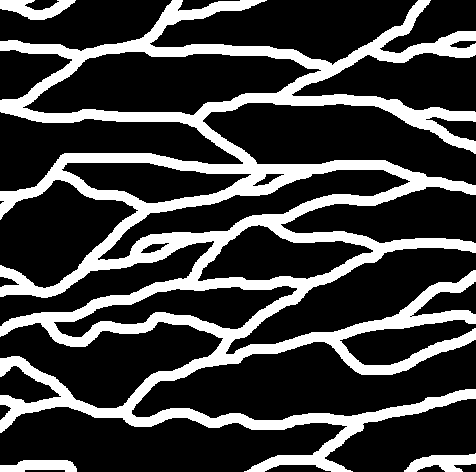
\includegraphics[scale=0.3]{channels}
			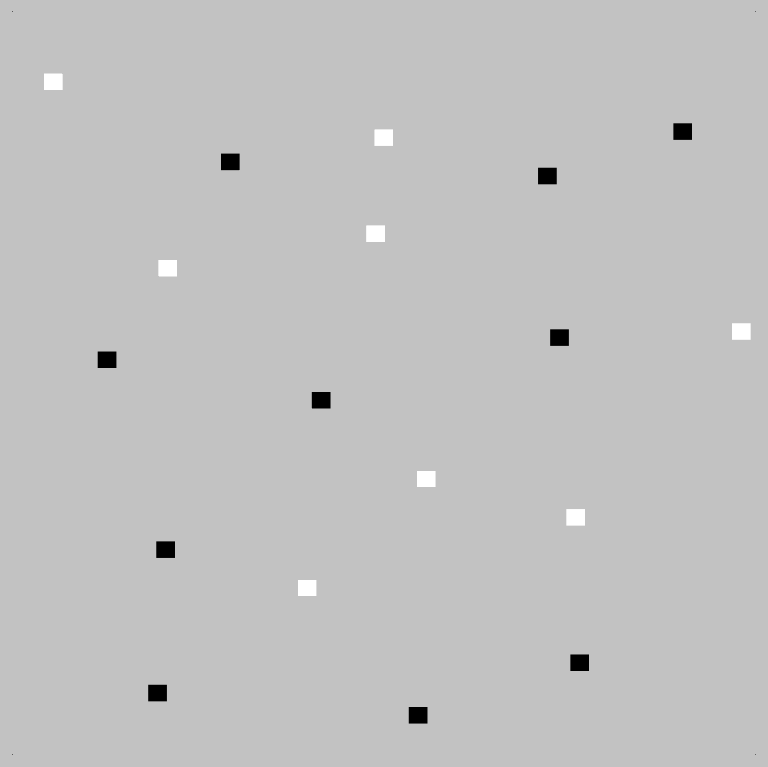
\includegraphics[scale=0.25]{cons}
			\caption{a) A Data sampled from our dataset, b) A constraint obtained from a sampled data and a mask}
			\label{channels}
		\end{figure}
	
	\subsection{Naming conventions}
	
		From now on, we will use the following naming conventions :
		
		\begin{itemize}
			
			\item $\mathop{\mathbb{{P}}_{r}}$ the real-data distribution : $x\sim \mathop{\mathbb{{P}}_{r}}, x\in M_{m, n}$
			
			\item $\mathop{\mathbb{{P}}_{z}}$ a "classical" distribution (in most cases, an uniform distribution $U[0,1]^n$)
			
			\item $\mathop{\mathbb{{P}}_{m}}$ the distribution in which the constraint masks will be sampled (\ref{constraints}) $m \sim 
			\mathop{\mathbb{{P}}_{m}},  m \in \{0, 1\}^{n\times n}$
			
			\item $c$ a shortcut for $x\sim \mathop{\mathbb{{P}}_{r}},	m \sim \mathop{\mathbb{{P}}_{m} } m\odot x$. We will note $ \mathop{\mathbb{{P}}_{c} }$ the distribution of  $c$ with respect to $\mathop{\mathbb{{P}}_{r}}$ and $ \mathop{\mathbb{{P}}_{m} }$.
			
		\end{itemize}

\section{Background}

	\subsection{Generative Adversarial Networks}
	
		Generative Adversarial Networks\cite{goodfellow14} are a method for training generative neural networks in an unsupervised way. It consists in a game between a generator $G$ and a discriminator network $D$, in which the generator learns to produce new data and discriminator learns to distinguish real examples from generated ones.
		
		More formally, training GANs is equivalent to solving the following minimax game :
		
		\begin{equation}
			\min_G \max_D L(D, G) = \mathop{\mathbb{E}}_{x\sim P_r} [\log (D(x))] + \mathop{\mathbb{E}}_{z\sim P_z} [\log (1-D(G(z)))]
		\end{equation}
		
		From this problem, one can derive a loss function for both the generator and the discriminator and find that minimizing those losses is equivalent to solving the minimax game, as well as minimizing the Kullback-Leibler divergence between the real-data distribution and the distribution of samples which can be generated by $G$. 
		
		In this document, we will focus on a more recent approach, the Wasserstein GAN (\cite{arjovski2017}), in which the problem is reformulated to minimize an Earth-Mover distance instead of the KL divergence. This new problem can be formulated as :
		
		\begin{equation}
			\min_G \max_D L(D, G) = \mathop{\mathbb{E}}_{x\sim P_r} [D(x)] + \mathop{\mathbb{E}}_{z\sim P_z} [1-D(G(z))]
		\end{equation}
		
		From this formulation, we can derive the  the following loss fuctions, which we will use as our objectives :
		
		\begin{equation}
			L_{D} =  \mathop{\mathbb{E}}_{x\sim P_r} [D(x)] - \mathop{\mathbb{E}}_{z\sim P_z} [D(G(z))]
		\end{equation}
		
		\begin{equation}
			L_{G} = -\mathop{\mathbb{E}}_{z\sim P_z} [D(G(z))]
		\end{equation}
	
	\subsection{Spatial Generative Adversarial Networks}
		
		Spacial Generative Adversarial Networks (SGANs)\cite{Jetchev} are a category of GANs in which both the generator and the discriminator nets are fully-convolutional networks. This characteristic brings several specificities. First, the networks are unable to pick up global dependencies in the data, because the total size of the data is greater than the total receptive field of the networks. Then, the output is not a single scalar, but a matrix of values. so the new objective becomes the mean of the discriminator's output :		
		
		\begin{equation}
			\min_G \max_D L(D, G) = \mathop{\mathbb{E}}_{x\sim P_r} [\frac{1}{m}\sum_{i=1}^{m} (D(x))] + \mathop{\mathbb{E}}_{z\sim P_z} [\frac{1}{m}\sum_{i=1}^{m}  (1-D(G(z)))]
		\end{equation}
		
		Despite their inability to pick up global dependencies in the data, SGANs have several advantages over the regular GANs. First, because dense layers usually contains the majority of the network's weights, SGAN have far less parameters than more classical GANs. Then, as both of the networks are fully-convolutional, there is no restrictions over the size or shape of the input, as long as it keeps the same number of dimensions.
		
	
	\subsection{Conditional Generative Adversarial Networks}
	
		Conditional Generative Adversarial Networks\cite{mirza14} are a subclass of GANs in which some additional information $y$ is given to both the generator and the discriminator as an input. This allows the conditioning of the generator without changing anything else in the learning algorithm.
		
		\begin{equation}
		\min_G \max_D L(D, G) = \mathop{\mathbb{E}}_{\substack{y\sim P_{y}\\x\sim P_{r|k} }} [(D(x | y))] + \mathop{\mathbb{E}}_{\substack{\tilde{y}\sim P_{y}\\z\sim P_z}} [ (1-D(G(z | \tilde{y}) | \tilde{y}))]
		\end{equation}

		
\section{Generative Adversarial Networks under spatial constraints}

	In this section, we will present the different three approaches we introduced to tackle this problem. We first introduce various objectives, derived from the original GAN formulation, which will be optimized in our approaches. We will then introduce  an unsupervised approach, where the constraints are only additional inputs of both the generator and the discriminator and finally, we present a supervised approach in which a cost between the constraints and the generated data is explicitly added to the generator's objective. 
	
	\subsection{Integrating constraints to the objectives}
	
		Our first approach is the spacial counterpart to the CGAN approach  for constraining GANs. In this approach, the constraints are given to both of the networks as another input matrix and the standard GAN objective becomes :
	
		\begin{equation}
			\label{cgan}
			L_{D}  = \mathop{\mathbb{{E}}_{\substack{
						x \sim \mathop{\mathbb{{P}}_{r}} \\
						m \sim \mathop{\mathbb{{P}}_{m}}
			}}} [D(x, m\odot x)] 
			- \mathop{\mathbb{{E}}}_{\substack{
					\tilde{x} \sim \mathop{\mathbb{{P}}_{r}} \\
					\tilde{m} \sim \mathop{\mathbb{{P}}_{m} }\\
					z \sim \mathop{\mathbb{{P}}_{z} }
			}} [D(G(z, \tilde{m}\odot\tilde{x}), \tilde{m}\odot\tilde{x})] 
		\end{equation}
		
		\begin{equation}
			L_{G}  = \mathop{\mathbb{{E}}}_{\substack{
					z \sim \mathop{\mathbb{{P}}_{z}} \\
					\tilde{x} \sim \mathop{\mathbb{{P}}_{r}} \\
					\tilde{m} \sim \mathop{\mathbb{{P}}_{m} }
			}} [D(G(z, \tilde{m}\odot\tilde{x}))] 
		\end{equation}
	
		A second type of approach consists in training the generator to respect constraints by adding an explicit cost to the generator's objective, while still training it to generate data which are close to the real data distribution in an unsupervised way. This cost is a mean squared error between the values of the generated data at the constrained points and the constraint :
	
		\begin{equation}
		\label{lc}
		L_C = \mathop{\mathbb{{E}}_{\substack{
					\hat{x} \sim \mathop{\mathbb{{P}}_{r}} \\
					\hat{z} \sim \mathop{\mathbb{{P}}_{z}}\\
					\hat{m} \sim \mathop{\mathbb{{P}}_{z}} \\	
		}}} || \hat{m} \odot \hat{x} - \hat{m} \odot G(\hat{z}, \hat{m} \odot \hat{x}) ||_2
		\end{equation}
		

		We then can add this new objective as a penalty on the generator's cost :

		
		\begin{equation}
		L_{G'} =  \mathop{\mathbb{{E}}}_{\substack{
				z \sim \mathop{\mathbb{{P}}_{z}} \\
				\tilde{x} \sim \mathop{\mathbb{{P}}_{r}} \\
				\tilde{m} \sim \mathop{\mathbb{{P}}_{m} }
		}} [D(G(z, \tilde{m}\odot\tilde{x}))]  + \lambda L_C
		\end{equation}

		Note that this objective is compatible with the unsupervised approach, as the constraints can be fed to the discriminator or not. In that case, the objectives become :
	
		\begin{equation}
		L_{D} =  \mathop{\mathbb{E}}_{\substack{
				x\sim \mathop{\mathbb{P}_r}\\	
				m \sim \mathop{\mathbb{P}}_{m}}}
		[D(x, m\odot x)] - \mathop{\mathbb{{E}}}_{\substack{
				z \sim \mathop{\mathbb{{P}}_{z}} \\
				\tilde{x} \sim \mathop{\mathbb{{P}}_{r}} \\
				\tilde{m} \sim \mathop{\mathbb{{P}}_{m} }
		}} [D(G(z, \tilde{m}\odot\tilde{x}), \tilde{m}\odot\tilde{x})] 
		\end{equation}
		
		
		\begin{equation}
		L_{G} =  \mathop{\mathbb{{E}}}_{\substack{
				z \sim \mathop{\mathbb{{P}}_{z}} \\
				\tilde{x} \sim \mathop{\mathbb{{P}}_{r}} \\
				\tilde{m} \sim \mathop{\mathbb{{P}}_{m} }
		}} [D(G(z, \tilde{m}\odot\tilde{x}), \tilde{m}\odot\tilde{x})]  + \lambda L_C
		\end{equation}
		
	
	\subsection{Learning with constraints}
	
		From these objectives, we derive several GAN formulations that integrates constraints. 	We first present the unsupervised approach, inherited from CGAN and optimizing the objective defined in \eqref{cgan} :
	
		\begin{align}
			\min_G \max_D  L(D, G) = \mathop{\mathbb{{E}}_{\substack{
						x \sim \mathop{\mathbb{{P}}_{r}} \\
						m \sim \mathop{\mathbb{{P}}_{m}}
			}}} [D(x, m\odot x)] 
			- \mathop{\mathbb{{E}}}_{\substack{
					\tilde{x} \sim \mathop{\mathbb{{P}}_{r}} \\
					\tilde{m} \sim \mathop{\mathbb{{P}}_{m} }\\
					z \sim \mathop{\mathbb{{P}}_{z} }
			}} [D(G(z, \tilde{m}\odot\tilde{x}), \tilde{m}\odot\tilde{x})] 
		\end{align}
		
		Then, we propose the following approaches which introduce the explicit cost \eqref{lc} added to the generator. This cost can be added as a penalty term with a weight $\lambda$ :
		
		\begin{align}
			\min_G\max_D L(D, G)  &= \mathop{\mathbb{{E}}_{\substack{
						x \sim \mathop{\mathbb{{P}}_{r}} 
			}}} [D(x)] 
			- \mathop{\mathbb{{E}}}_{\substack{
					\tilde{x} \sim \mathop{\mathbb{{P}}_{r}} \\
					\tilde{m} \sim \mathop{\mathbb{{P}}_{m} }\\
					z \sim \mathop{\mathbb{{P}}_{z} }
			}} [D(G(z, \tilde{m}\odot\tilde{x}))]   \nonumber \\
		& + \lambda \mathop{\mathbb{{E}}_{\substack{
					\hat{x} \sim \mathop{\mathbb{{P}}_{r}} \\
					\hat{z} \sim \mathop{\mathbb{{P}}_{z}}\\
					\hat{m} \sim \mathop{\mathbb{{P}}_{z}} \\	
		}}} || \hat{m} \odot \hat{x} - \hat{m} \odot G(\hat{z}, \hat{m} \odot \hat{x}) ||_2
		\end{align}

		Another solution is to optimize the explicit cost function separately, forming a multi-objective problem : 

		\begin{equation}
		\left\{  \begin{split}
			& \min_G \max_D L(D, G)  = \mathop{\mathbb{{E}}_{\substack{
						x \sim \mathop{\mathbb{{P}}_{r}} \\
						m \sim \mathop{\mathbb{{P}}_{m}}
			}}} [D(x)] 
			- \mathop{\mathbb{{E}}}_{\substack{
					\tilde{x} \sim \mathop{\mathbb{{P}}_{r}} \\
					\tilde{m} \sim \mathop{\mathbb{{P}}_{m} }\\
					z \sim \mathop{\mathbb{{P}}_{z} }
			}} [D(G(z, \tilde{m}\odot\tilde{x}))] \\
			& \min_G L_C(G) = \mathop{\mathbb{{E}}_{\substack{
						\hat{x} \sim \mathop{\mathbb{{P}}_{r}} \\
						\hat{z} \sim \mathop{\mathbb{{P}}_{z}}\\
						\hat{m} \sim \mathop{\mathbb{{P}}_{z}} \\	
			}}} || \hat{m} \odot \hat{x} - \hat{m} \odot G(\hat{z}, \hat{m} \odot \hat{x}) ||_2
		 \end{split}\right.
		\end{equation}
		
		Finally, we can merge both of these approaches by giving the constraints as an input to the discriminator and adding the explicit objective :
		
			\begin{align}
		\min_G \max_D L(D, G)  &= \mathop{\mathbb{{E}}_{\substack{
					x \sim \mathop{\mathbb{{P}}_{r}} \\
					m \sim \mathop{\mathbb{{P}}_{m}}
		}}} [D(x, m\odot x)] 
		- \mathop{\mathbb{{E}}}_{\substack{
				\tilde{x} \sim \mathop{\mathbb{{P}}_{r}} \\
				\tilde{m} \sim \mathop{\mathbb{{P}}_{m} }\\
				z \sim \mathop{\mathbb{{P}}_{z} }
		}} [D(G_\theta(z, \tilde{m}\odot\tilde{x}), \tilde{m}\odot\tilde{x})]   \nonumber \\
		& + \lambda \mathop{\mathbb{{E}}_{\substack{
					\hat{x} \sim \mathop{\mathbb{{P}}_{r}} \\
					\hat{z} \sim \mathop{\mathbb{{P}}_{z}}\\
					\hat{m} \sim \mathop{\mathbb{{P}}_{z}} \\	
		}}} || \hat{m} \odot \hat{x} - \hat{m} \odot G(\hat{z}, \hat{m} \odot \hat{x}) ||_2
		\end{align}
		
		\begin{equation}
			\left\{  \begin{split}
			& \min_G \max_D L(D, G)  = \mathop{\mathbb{{E}}_{\substack{
						x \sim \mathop{\mathbb{{P}}_{r}} \\
						m \sim \mathop{\mathbb{{P}}_{m}}
			}}} [D(x, m\odot x)] 
			- \mathop{\mathbb{{E}}}_{\substack{
					\tilde{x} \sim \mathop{\mathbb{{P}}_{r}} \\
					\tilde{m} \sim \mathop{\mathbb{{P}}_{m} }\\
					z \sim \mathop{\mathbb{{P}}_{z} }
			}} [D(G(z, \tilde{m}\odot\tilde{x}), \tilde{m}\odot \tilde{x})] \\
			& \min_G L_C(G) = \mathop{\mathbb{{E}}_{\substack{
						\hat{x} \sim \mathop{\mathbb{{P}}_{r}} \\
						\hat{z} \sim \mathop{\mathbb{{P}}_{z}}\\
						\hat{m} \sim \mathop{\mathbb{{P}}_{z}} \\	
			}}} || \hat{m} \odot \hat{x} - \hat{m} \odot G(\hat{z}, \hat{m} \odot \hat{x}) ||_2
			\end{split}\right.
	\end{equation}		

\section{Network architectures}

	In this section, we will present the different architectures we came with for both the supervised and the unsupervised approach. Those architectures are fully-convolutional and have a similar number of parameters (around 8 million). The constraint is added as additional channels for both the generator and the discriminator.
	
	The different generators are made from transposed convolutional (also called deconvolution)  layers, with ReLU activations. BatchNorm\cite{ioffe15} is added between each layers, with the exception of the last layer. All the upscaling is done with striding ($1/2$ per layer).
	
	The discriminator is the same as \cite{jetchev}, which is itself a fully-convolutional adaptation of the DGCAN\cite{chintala14} discriminator. It consists in five convolutional layers with with LeakyReLU activations (except for the last one which has a sigmoid activation) and BatchNorm between all the layers except after the first layer and before the last one. Each layer has a striding of $2$, allowing downscaling without pooling.
		
	\subsection{Dilatation only}
	
		This architecture uses dilated convolutions (or "atrous" convolutions) and keeps both the input noise and the constraint to the same constant size
		
	\subsection{Encoder-decoder}
	\subsection{Encoder-decoder with upscaling}
	\subsection{Upscaling and dilatation}
	\subsection{Encoder-decoder with noise encoding}

\section{Learning constraints by gradient descent in the noise}

	This is done by backpropagating the gradients of the previous cost through the generator and optimizing it with gradient descent
	A venir ?


\newpage
\section{Appendix}

	\subsection{Network architectures diagrams}
	
		\begin{figure}
			\centering
			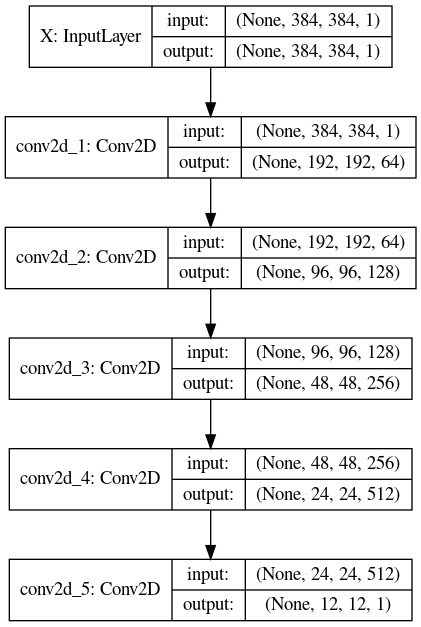
\includegraphics[scale=0.4]{discriminator.png}
			\caption{Discriminator}
		\end{figure}
	
		\begin{figure}
		\centering
		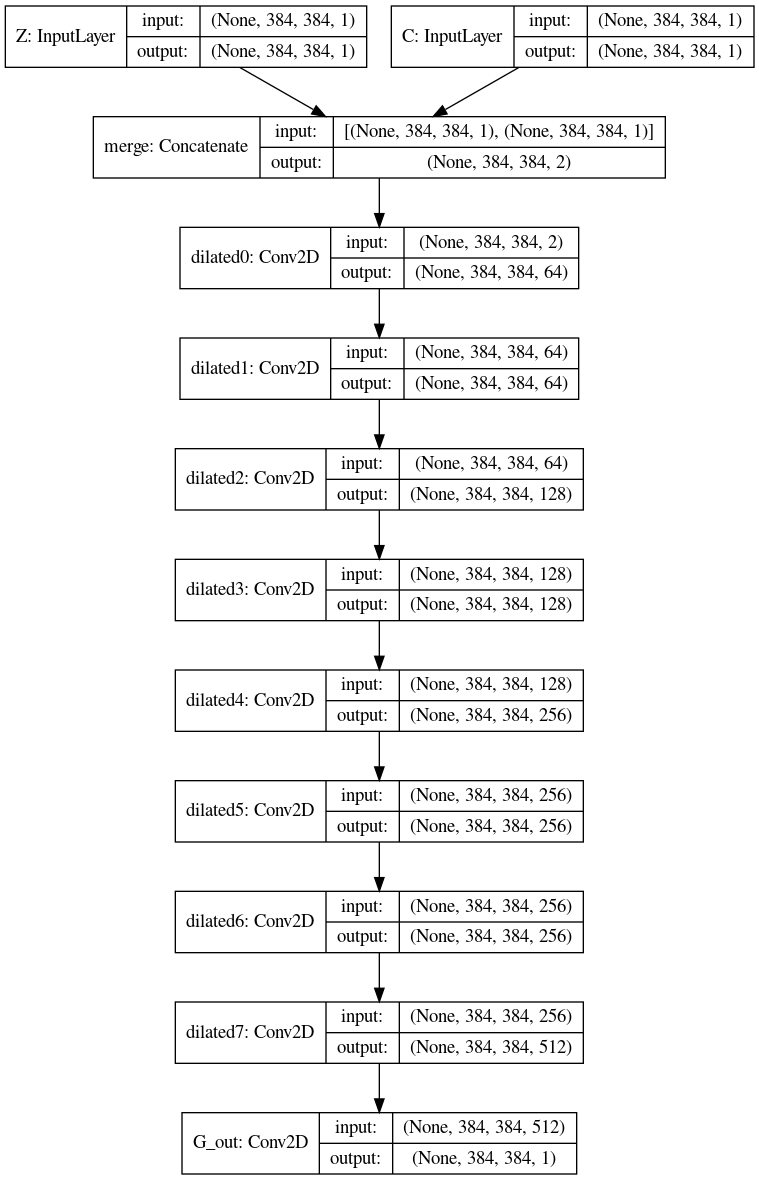
\includegraphics[scale=0.4]{dilated_only.png}
		\caption{Dilatation only}
		\end{figure}

	
		\begin{figure}
			\centering
			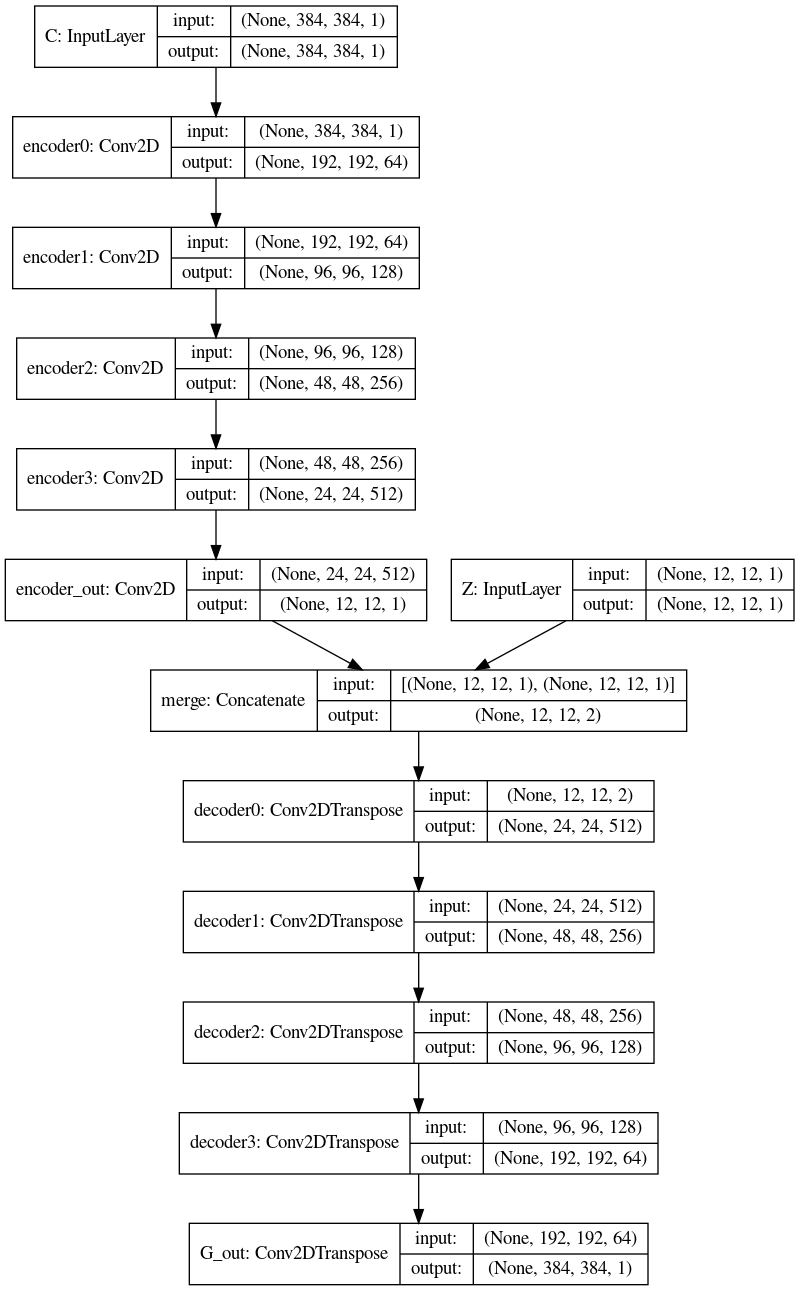
\includegraphics[scale=0.45]{encoder_decoder.png}
			\caption{Encoder-decoder}
		\end{figure}
	
		\begin{figure}
			\centering
			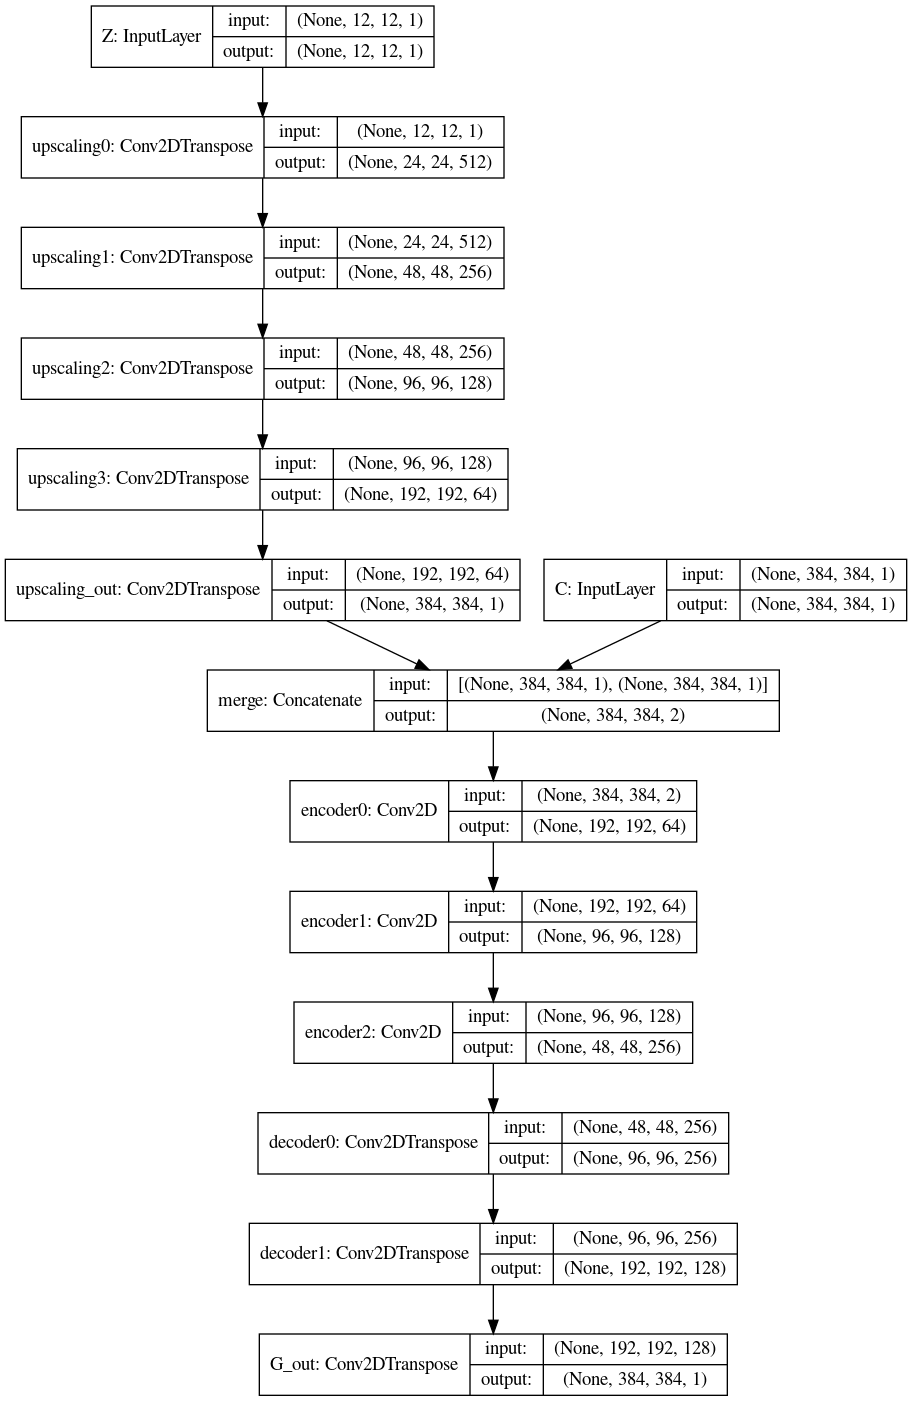
\includegraphics[scale=0.4]{upscaling_encoder_decoder.png}
			\caption{Encoder-decoder with upscaling}
		\end{figure}
	
		\begin{figure}
		\centering
		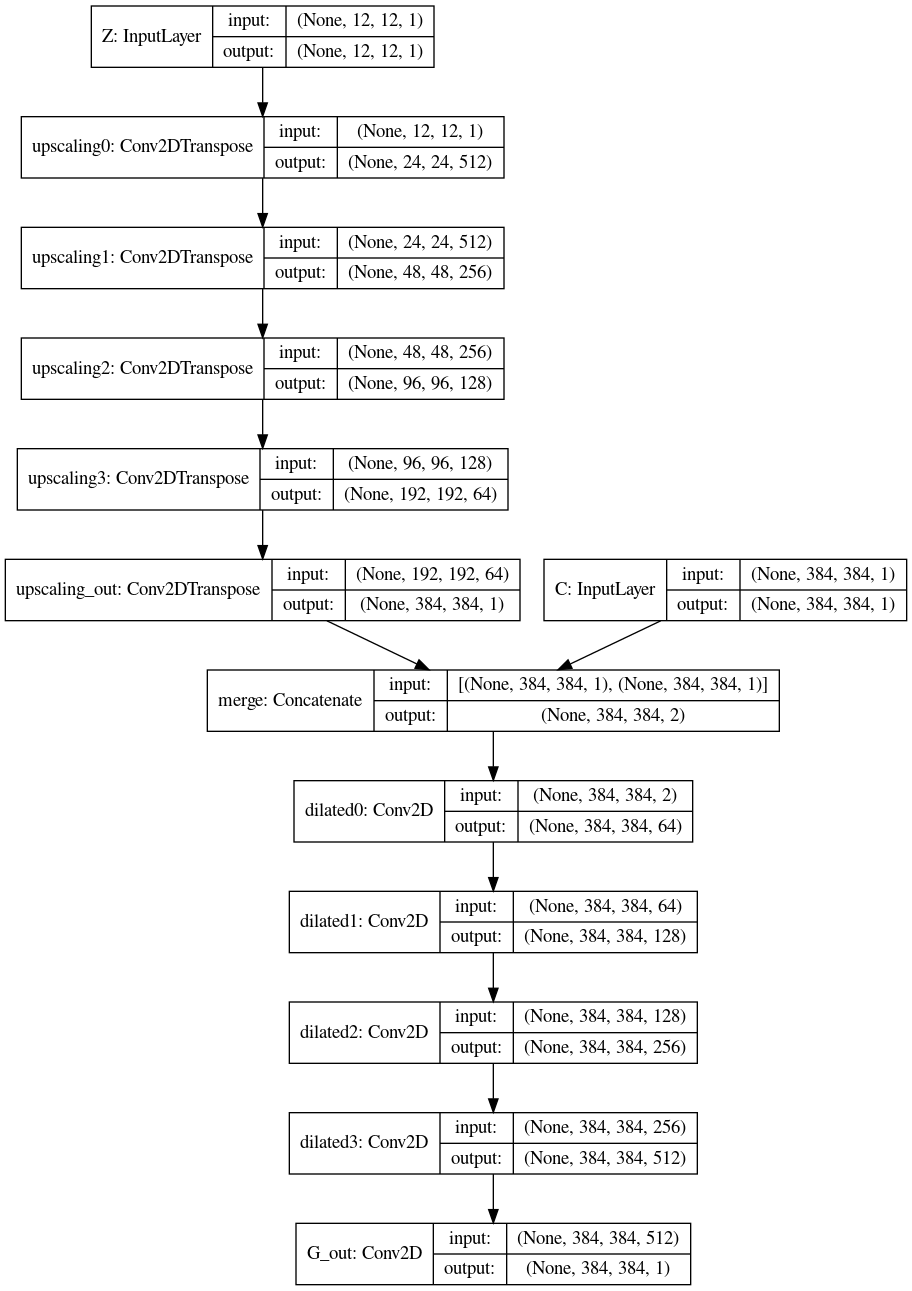
\includegraphics[scale=0.45]{upscaling_dilated.png}
		\caption{Upscaling and dilatation}
		\end{figure}
	
		\begin{figure}
		\centering
		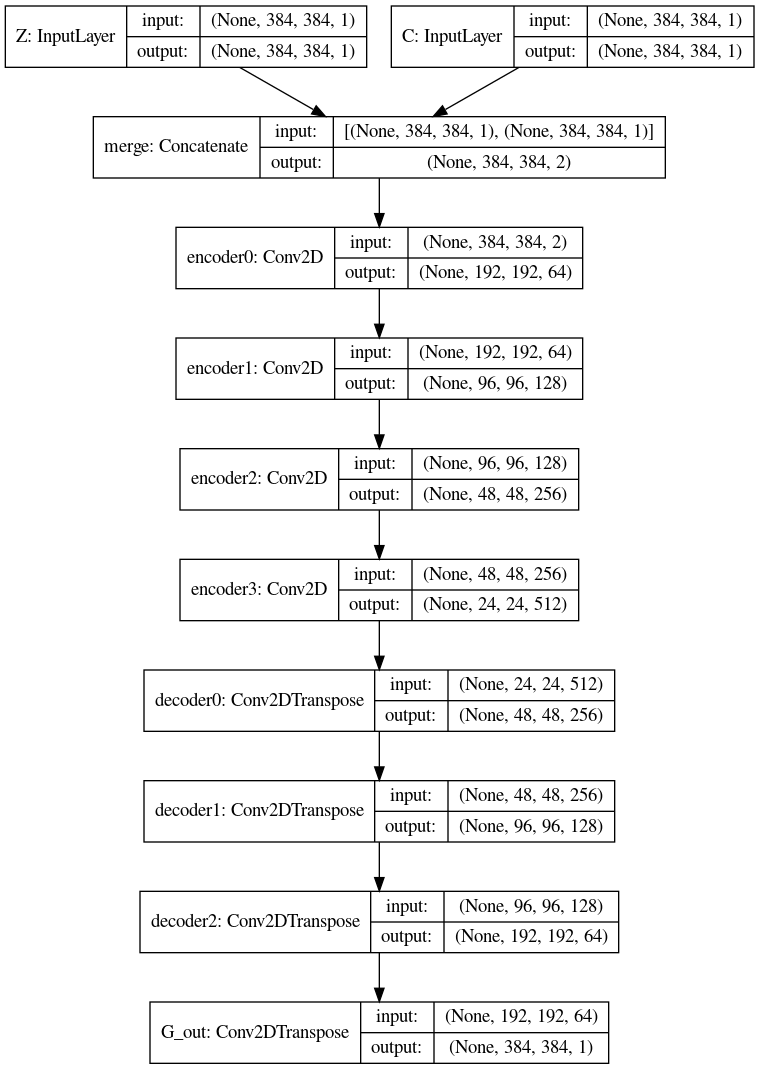
\includegraphics[scale=0.45]{encoder_decoder_large_noise.png}
		\caption{Encoder decoder with large noise}
		\end{figure}

	\subsection{Reformulation with a constraint variable}
	
		\subsection{Integrating constraints to the objectives}
	
	Our first approach is the spacial counterpart to the CGAN approach  for constraining GANs. In this approach, the constraints are given to both of the networks as another input matrix and the standard GAN objective becomes :
	
	\begin{equation}
	\label{cgan}
	L_{D}  = \mathop{\mathbb{{E}}_{\substack{
				x \sim \mathop{\mathbb{{P}}_{r}} \\
				m \sim \mathop{\mathbb{{P}}_{m}}\\
				c \sim \mathop{\mathbb{{P}}_{c}}(m, x)
	}}} [D(x, c)] 
	- \mathop{\mathbb{{E}}}_{\substack{
			\tilde{x} \sim \mathop{\mathbb{{P}}_{r}} \\
			\tilde{m} \sim \mathop{\mathbb{{P}}_{m} }\\
			z \sim \mathop{\mathbb{{P}}_{z} }\\
			\tilde{c} \sim \mathop{\mathbb{{P}}_{c}}(\tilde{m}, \tilde{x})
	}} [D(G(z, \tilde{c}), \tilde{c})] 
	\end{equation}
	
	\begin{equation}
	L_{G}  = \mathop{\mathbb{{E}}}_{\substack{
			z \sim \mathop{\mathbb{{P}}_{z}} \\
			\tilde{x} \sim \mathop{\mathbb{{P}}_{r}} \\
			\tilde{m} \sim \mathop{\mathbb{{P}}_{m} }\\
			c \sim \mathop{\mathbb{{P}}_{c}}(m, x)
	}} [D(G(z, \tilde{c}))] 
	\end{equation}
	
	A second type of approach consists in training the generator to respect constraints by adding an explicit cost to the generator's objective, while still training it to generate data which are close to the real data distribution in an unsupervised way. This cost is a mean squared error between the values of the generated data at the constrained points and the constraint :
	
	\begin{equation}
	\label{lc}
	L_C = \mathop{\mathbb{{E}}_{\substack{
				\hat{x} \sim \mathop{\mathbb{{P}}_{r}} \\
				\hat{z} \sim \mathop{\mathbb{{P}}_{z}}\\
				\hat{m} \sim \mathop{\mathbb{{P}}_{z}} \\	
				\hat{c} \sim \mathop{\mathbb{{P}}_{c}}(\tilde{m}, \tilde{x})
	}}} || \hat{c} - \hat{m} \odot G(\hat{z}, \hat{c}) ||_2
	\end{equation}
	
	
	We then can add this new objective as a penalty on the generator's cost :
	
	
	\begin{equation}
	L_{G'} =  \mathop{\mathbb{{E}}}_{\substack{
			z \sim \mathop{\mathbb{{P}}_{z}} \\
			\tilde{x} \sim \mathop{\mathbb{{P}}_{r}} \\
			\tilde{m} \sim \mathop{\mathbb{{P}}_{m} }\\
			\tilde{c} \sim \mathop{\mathbb{{P}}_{c}}(\tilde{m}, \tilde{x})
	}} [D(G(z, \tilde{c}))]  + \lambda L_C
	\end{equation}
	
	Note that this objective is compatible with the unsupervised approach, as the constraints can be fed to the discriminator or not. In that case, the objectives become :
	
	\begin{equation}
	L_{D} =  \mathop{\mathbb{E}}_{\substack{
			x\sim \mathop{\mathbb{P}_r}\\	
			m \sim \mathop{\mathbb{P}}_{m}\\
			c \sim \mathop{\mathbb{{P}}_{c}}(m, x)}}
	[D(x, c)] - \mathop{\mathbb{{E}}}_{\substack{
			z \sim \mathop{\mathbb{{P}}_{z}} \\
			\tilde{x} \sim \mathop{\mathbb{{P}}_{r}} \\
			\tilde{m} \sim \mathop{\mathbb{{P}}_{m} }\\
			\tilde{c} \sim \mathop{\mathbb{{P}}_{c}}(\tilde{m}, \tilde{x})
	}} [D(G(z, \tilde{c}), \tilde{c})] 
	\end{equation}
	
	
	\begin{equation}
	L_{G} =  \mathop{\mathbb{{E}}}_{\substack{
			z \sim \mathop{\mathbb{{P}}_{z}} \\
			\tilde{x} \sim \mathop{\mathbb{{P}}_{r}} \\
			\tilde{m} \sim \mathop{\mathbb{{P}}_{m} }\\
			\tilde{c} \sim \mathop{\mathbb{{P}}_{c}}(\tilde{m}, \tilde{x})
	}} [D(G(z, \tilde{c}), \tilde{c})]  + \lambda L_C
	\end{equation}
	
	
	\subsection{Learning with constraints}
	
	From these objectives, we derive several GAN formulations that integrates constraints. 	We first present the unsupervised approach, inherited from CGAN and optimizing the objective defined in \eqref{cgan} :
	
	\begin{align}
	\min_G \max_D  L(D, G) = \mathop{\mathbb{{E}}_{\substack{
				x \sim \mathop{\mathbb{{P}}_{r}} \\
				m \sim \mathop{\mathbb{{P}}_{m}}\\
				c \sim \mathop{\mathbb{{P}}_{c}}(m, x)
	}}} [D(x, c)] 
	- \mathop{\mathbb{{E}}}_{\substack{
			\tilde{x} \sim \mathop{\mathbb{{P}}_{r}} \\
			\tilde{m} \sim \mathop{\mathbb{{P}}_{m} }\\
			z \sim \mathop{\mathbb{{P}}_{z} }\\
			\tilde{c} \sim \mathop{\mathbb{{P}}_{c}}(\tilde{m}, \tilde{x})
	}} [D(G(z, \tilde{c}), \tilde{c})] 
	\end{align}
	
	Then, we propose the following approaches which introduce the explicit cost \eqref{lc} added to the generator. This cost can be added as a penalty term with a weight $\lambda$ :
	
	\begin{align}
	\min_G\max_D L(D, G)  &= \mathop{\mathbb{{E}}_{\substack{
				x \sim \mathop{\mathbb{{P}}_{r}} 
	}}} [D(x)] 
	- \mathop{\mathbb{{E}}}_{\substack{
			\tilde{x} \sim \mathop{\mathbb{{P}}_{r}} \\
			\tilde{m} \sim \mathop{\mathbb{{P}}_{m} }\\
			z \sim \mathop{\mathbb{{P}}_{z} }\\
			\tilde{c} \sim \mathop{\mathbb{{P}}_{c}}(\tilde{m}, \tilde{x})
	}} [D(G(z, \tilde{c}))]   \nonumber \\
	& + \lambda \mathop{\mathbb{{E}}_{\substack{
				\hat{x} \sim \mathop{\mathbb{{P}}_{r}} \\
				\hat{z} \sim \mathop{\mathbb{{P}}_{z}}\\
				\hat{m} \sim \mathop{\mathbb{{P}}_{z}} \\	
				\hat{c} \sim \mathop{\mathbb{{P}}_{c}}(\hat{m}, \hat{x})
	}}} || \hat{c} - \hat{m} \odot G(\hat{z}, \hat{c}) ||_2
	\end{align}
	
	Another solution is to optimize the explicit cost function separately, forming a multi-objective problem : 
	
	\begin{equation}
	\left\{  \begin{split}
	& \min_G \max_D L(D, G)  = \mathop{\mathbb{{E}}_{\substack{
				x \sim \mathop{\mathbb{{P}}_{r}} \\
				m \sim \mathop{\mathbb{{P}}_{m}}\\
				c \sim \mathop{\mathbb{{P}}_{c}}(m, x)
	}}} [D(x)] 
	- \mathop{\mathbb{{E}}}_{\substack{
			\tilde{x} \sim \mathop{\mathbb{{P}}_{r}} \\
			\tilde{m} \sim \mathop{\mathbb{{P}}_{m} }\\
			\tilde{c} \sim \mathop{\mathbb{{P}}_{c}}(\tilde{m}, \tilde{x})\\
			z \sim \mathop{\mathbb{{P}}_{z} }
	}} [D(G(z, \tilde{c}))] \\
	& \min_G L_C(G) = \mathop{\mathbb{{E}}_{\substack{
				\hat{x} \sim \mathop{\mathbb{{P}}_{r}} \\
				\hat{z} \sim \mathop{\mathbb{{P}}_{z}}\\
				\hat{m} \sim \mathop{\mathbb{{P}}_{z}} \\	
				\hat{c} \sim \mathop{\mathbb{{P}}_{c}}(\hat{m}, \hat{x})
	}}} || \hat{c} - \hat{m} \odot G(\hat{z}, \hat{c}) ||_2
	\end{split}\right.
	\end{equation}
	
	Finally, we can merge both of these approaches by giving the constraints as an input to the discriminator and adding the explicit objective :
	
	\begin{align}
	\min_G \max_D L(D, G)  &= \mathop{\mathbb{{E}}_{\substack{
				x \sim \mathop{\mathbb{{P}}_{r}} \\
				m \sim \mathop{\mathbb{{P}}_{m}} \\
				c \sim \mathop{\mathbb{{P}}_{c}}(m, x)
	}}} [D(x, c)] 
	- \mathop{\mathbb{{E}}}_{\substack{
			\tilde{x} \sim \mathop{\mathbb{{P}}_{r}} \\
			\tilde{m} \sim \mathop{\mathbb{{P}}_{m} }\\
			\tilde{c} \sim \mathop{\mathbb{{P}}_{c}}(\tilde{m}, \tilde{x})\\
			z \sim \mathop{\mathbb{{P}}_{z} }
	}} [D(G_\theta(z, \tilde{c}), \tilde{c})]   \nonumber \\
	& + \lambda \mathop{\mathbb{{E}}_{\substack{
				\hat{x} \sim \mathop{\mathbb{{P}}_{r}} \\
				\hat{z} \sim \mathop{\mathbb{{P}}_{z}}\\
				\hat{m} \sim \mathop{\mathbb{{P}}_{z}} \\	
				\hat{c} \sim \mathop{\mathbb{{P}}_{c}}(\hat{m}, \hat{x})
	}}} || \hat{c} - \hat{m} \odot G(\hat{z}, \hat{c}) ||_2
	\end{align}
	
	\begin{equation}
	\left\{  \begin{split}
	& \min_G \max_D L(D, G)  = \mathop{\mathbb{{E}}_{\substack{
				x \sim \mathop{\mathbb{{P}}_{r}} \\
				m \sim \mathop{\mathbb{{P}}_{m}}\\
				c \sim \mathop{\mathbb{{P}}_{c}}(m, x)
	}}} [D(x, c)] 
	- \mathop{\mathbb{{E}}}_{\substack{
			\tilde{x} \sim \mathop{\mathbb{{P}}_{r}} \\
			\tilde{m} \sim \mathop{\mathbb{{P}}_{m} }\\
			\tilde{c} \sim \mathop{\mathbb{{P}}_{c}}(\tilde{m}, \tilde{x})\\
			z \sim \mathop{\mathbb{{P}}_{z} }
	}} [D(G(z, \tilde{c}), \tilde{c})] \\
	& \min_G L_C(G) = \mathop{\mathbb{{E}}_{\substack{
				\hat{x} \sim \mathop{\mathbb{{P}}_{r}} \\
				\hat{z} \sim \mathop{\mathbb{{P}}_{z}}\\
				\hat{m} \sim \mathop{\mathbb{{P}}_{z}} \\	
				\hat{c} \sim \mathop{\mathbb{{P}}_{c}}(\hat{m}, \hat{x})
	}}} || \hat{c} - \hat{m} \odot G(\hat{z}, \hat{c}) ||_2
	\end{split}\right.
	\end{equation}		

\end{document}